\documentclass[12pt,a4paper]{monografia}
\usepackage{amsfonts}
\usepackage{amsmath}


%TODOS OS PACKAGE DEVEM SER COLOCADOS AKI
\usepackage[brazil,brazilian,portuges]{babel}
\usepackage[T1]{fontenc}
%\usepackage[brazilian]{babel}
\usepackage{times}
\usepackage{amsmath,listings,indentfirst,url,hyperref}
%\usepackage{amsmath,listings,indentfirst}
\usepackage{paralist}
\usepackage[all]{hypcap}
\usepackage{paralist}
\usepackage{subfigure,comment}
\usepackage[alf]{abntcite}
\usepackage[portuguese]{nomencl}
\usepackage{longtable}
\usepackage{fancyvrb}
\usepackage{color}
\usepackage{rotating}
\usepackage{multirow}
\usepackage{latexsym}
\usepackage [ table ]{xcolor}
\usepackage[utf8]{inputenc}
\usepackage[section]{placeins}
\usepackage{graphicx}


% pacotes de fontes! doi ter que usar times para evitar problemas :(
%\usepackage{fontspec}
%\usepackage{xunicode} 
%\defaultfontfeatures{Mapping=tex-text} 
%\setromanfont{Garamond}
%\setsansfont{Gill Sans}
%\setmonofont{Courier New}

% Listings
\lstset{
    inputencoding=utf8,
    basicstyle=\scriptsize,
    frame=single,
	tabsize=4,
	captionpos=b,
	breaklines=true,
	numbers=left,
}

% Não sei porque mas o LaTeX insiste em avançar a margem nas citações.
% Felizmente há o comando \sloppy, que diz para aumentar o espaçamento
% entre as palavras, visando /sempre/ respeitar as margens. Fica feio
% em alguns parágrafos, mas é a vida...
\sloppy
\begin{comment}
\tolerance 1414
\hbadness 1414
\emergencystretch 1.5em
\hfuzz 0.3pt
\widowpenalty=10000
\vfuzz \hfuzz
\raggedbottom
\end{comment}

% da um trato nos floats
\renewcommand{\topfraction}{.85}
\renewcommand{\bottomfraction}{.7}
\renewcommand{\textfraction}{.15}
\renewcommand{\floatpagefraction}{.66}
\renewcommand{\dbltopfraction}{.66}
\renewcommand{\dblfloatpagefraction}{.66}
\setcounter{topnumber}{9}
\setcounter{bottomnumber}{9}
\setcounter{totalnumber}{20}
\setcounter{dbltopnumber}{9}

%\addto\captionsportuges{
%  \renewcommand{\tablename}
%    {Quadro}}

%\addto\captionsportuges{
%  \renewcommand{\listtablename}
%    {Lista de Quadros}}

\renewcommand{\lstlistingname}{C\'odigo}
\def\listofsymbols{
\def\addsymbol #1 #2{#1  & \hspace{0.5in} #2 \\ } 

\begin{tabular}{l l}
	%\addsymbol UML {\textit{Unified Modeling Language}}
	%\addsymbol AM {Aprendizado de Máquina}
    \addsymbol GNS3 {Graphical Network Simulator 3 }
    \addsymbol WWW {World Wide Web}
    \addsymbol HTTP {Hypertext Transfer Protocol}
    \addsymbol HTTPS {Hypertext Transfer Protocol Secure}
    \addsymbol TCP {Transmission Control Protocol}
    \addsymbol IP { Internet Protocol }
    \addsymbol SSL {Secure Socket Layer}
\end{tabular}

 \clearpage}

% Verbatim não precisa de espaçamento duplo e nem de fontes tão grandes
\RecustomVerbatimEnvironment
	{Verbatim}%
	{Verbatim}%
	{baselinestretch=1,	fontsize=\relsize{-1}}



%%%%%%%%%%%%%%count enumarete start in zero
\usepackage{enumitem}
\setlist[enumerate,1]{start=1} % only outer nesting level

%%%%%%%%cite inside enumerate
\makeatletter
\newcommand{\mylabel}[2]{#2\def\@currentlabel{#2}\label{#1}}
\makeatother


\hyphenation{re-co-nhe-ci-men-to}
\hyphenation{re-su-mi-da-men-te}
\hyphenation{in-vá-li-da}
\hyphenation{i-ma-gem}
\hyphenation{li-te-ra-tu-ra}
\hyphenation{ma-nu-al-men-te}
\hyphenation{re-pre-sen-ta}
\begin{document}
	\titulo{ANÁLISE DO GNS3 COMO FERRAMENTA AUXILIAR AO ENSINO DO PROTOCOLO HTTP POR MEIO DA COMUNICAÇÃO ENTRE REDES SIMULADAS}
\autor{Christopher Renkavieski \\ Lucas Machado Gutierrez \\ Marlon Henry Schweigert}
\nome{Christopher\\Lucas\\ Marlon}
\ultimonome{Renkavieski \\ Gutierrez \\ Schweigert}

\bacharelado \curso{Ciência da Computação}
\ano{2016}
\data {\today}
\cidade{Joinville}

\instituicao{Universidade do Estado de Santa Catarina}
\sigla{UDESC}
\unidadeacademica{Centro de Ciências Tecnológicas}

\orientador{Prof\textordmasculine  Charles Christian Miers}
\examinadorum{Prof\textordmasculine  Charles Christian Miers}
\examinadordois{Prof\textordmasculine  Guilherme Piegas Koslovski}

\ttorientador{$ $}
\ttexaminadorum{$ $}
\ttexaminadordois{$ $}

\newpage
\pagestyle{empty}

\maketitle

%\begin{dedicatoria}
%\noindent
%\end{dedicatoria}
%\noindent
%\newpage
%\begin{epigrafe}
%\noindent
%"xxxxxxx"
%--alguem
%\end{epigrafe}

%\agradecimento{Agradecimentos}
%caneta



%\resumo{Resumo}

%Do momento de sua invenção até hoje, a Internet foi responsável por mudanças radicais e profundas na sociedade, permitindo comunicação e acesso a informação a taxas nunca antes experimentadas [ref: livro kurose e ross].
%A definição mais básica de internet é uma rede de redes. Já a Internet, com “I” maiúsculo, é uma rede de redes específica, que hoje conecta computadores, dispositivos móveis e outros por todo o planeta, tendo como base os protocolos de transmissão TCP/IP, e sobre a qual está edificada a World Wide Web (WWW).

%Para que a conexão entre as diversas redes da Internet seja possível, um dos conceitos fundamentais é o de roteamento, conectando os principais serviços desejados a todos os usuários desta enorme rede.

%[Continua]

%\noindent \textbf{Palavras-chave:} \textit{GNC3}, \textit{Simulação de Redes}, \textit{HTTP}, \textit{Análise de Redes Simuladas}.

%\resumo{Abstract}

%From the moment of its invention until today, the Internet was responsible for radical and profound changes in society, allowing communication and access to information at rates never before experienced [ref: book kurose and ross].
%The most basic definition of the internet is a network of networks. The Internet, with a capital "I", is a specific network of networks, which today connects computers, mobile devices and others across the globe, based on TCP / IP transmission protocols, and on which World is built Wide Web (WWW).

%In order for the connection between different Internet networks to be possible, one of the fundamental concepts is routing, connecting the main desired services to all users of this huge network.

%[Resumo Traduzido]

%\noindent \textbf{Palavras-chave:} \textit{GNS3}, \textit{Simulated Networks}, \textit{HTTP}, \textit{Simulated Network Analysis}.


\tableofcontents
\listoffigures
\listoftables
\newpage
\chapter*{Lista de Abreviaturas\hfill} \addcontentsline{toc}{chapter}{Lista de Abreviaturas}
\listofsymbols

\newpage
\pagestyle{myheadings}

	\chapter{Introdução}
\label{ch:intro}

O DNS (\textit{Domain Name System}) \cite{rfc1034} é um sistema
distribuído de resolução de nomes que desempenha um papel fundamental
na Internet. Sua principal funcionalidade é traduzir nomes de domínio
mais facilmente memorizáveis (como \url{www.udesc.br}) em endereços IP
numéricos (como 200.19.105.194), que são usados pelos protocolos
subjacentes de rede para localizar e identificar nós na Internet.

Em vista de sua ampla utilização, o DNS também é tanto um alvo quanto
um vetor de ataques. As principais ameaças envolvendo o DNS são
resumidas por \cite{Conrad:2012:tidssr}, que as divide em duas
classes, aquelas em que o DNS é o alvo e aquelas que são oportunizadas
pelo DNS\@. A classe de ameaças ao DNS inclui:

\begin{itemize}

\item Negação de serviço: impedir o acesso de usuários ao DNS, com isso
  prejudicando ou mesmo bloqueando o seu acesso à Internet;

\item Corrupção de dados: modificar dados publicados no DNS de forma
  não autorizada, o que pode, por exemplo, levar usuários a acessar
  sites ilegítimos (como páginas falsas de bancos ou comércio
  eletrônico);

\item Exposição de informação: revelar informações sobre o
  comportamento dos usuários, como histórico de sites web acessados \cite{cert3}.
\end{itemize}

O DNS também pode ser usado como um veículo de ataques. A classe de
ameaças oportunizadas pelo DNS abrange:

\begin{itemize}
\item Ataques de amplificação: servidores DNS mal configurados podem ser
  usados para realizar ataques de negação de serviço contra terceiros \cite{cert3};
  %[CERT.br, Servidores DNS recursivos abertos]

\item \textit{Fast flux} DNS: servidores usados para propósitos
  nefastos, como propagação de software malicioso ou controle remoto
  de \textit{botnets}, podem ter diversos endereços IP distintos
  associados. Uma fração desses endereços são associados a um nome DNS
  específico e trocados com alta frequência, de modo a dificultar a
  localização dos servidores e a identificação dos seus responsáveis,
  e até mesmo balancear carga entre servidores
  \cite{Salusky:2007:ffsn};

\item Exfiltração de dados: como o tráfego DNS geralmente não é
  barrado ou modificado por \textit{firewalls}, ele é usado com
  frequência para transmitir dados sensíveis (capturados no curso
  de uma invasão) sem que isso seja percebido pelos mecanismos de
  defesa da rede.
\end{itemize}  
  
O maior ataque DDoS foi registrado em setembro de 2016, que conseguiu alcançar picos de 1 Tbps de tráfego.

O serviço de hospedagem OVH (\textit{Hosted service provider company}) na França foi a vítima, dos ataques que conseguiu alcançar a marca de 1 Tbps por segundo, os ataques acabaram utilizando \textit{Smart Devices} para a realização dos ataques. Dispositivos inteligentes faziam parte da \textit{botnet} que foi utilizada para a realização dos ataques. 

Octave Klaba, o fundador e CTO (\textit{chief technology officer}) da OVH, apresentou os diversos ataques que foram realizados, e o volume de tráfego que excedia 100 Gbps e atingiam picos de 799 Gbps. O ataque foi realizado por mais de 152000 dispositivos da IoT (\textit{Internet of Things}), que incluíam câmeras e gravadores de vídeo comprometidos \cite{report:ddos}.


\iffalse 
%- O que é o DNS, qual o seu papel na Internet 
Apesar da grande popularização dos meios de pesquisa e viabilização de diferentes tarefas, como transações bancarias. A internet com mais de 1 bilão de usuários, ainda possui fatores desconhecidos por seus usuários \cite{radware}. 
%% i  try,

Um serviço de DNS (Domain Name System) é responsável pela tradução de um \textit{host name}, ao receber uma URL (\textit{Uniform Resource Locators}), será responsável pela sua tradução para um endereço \textit{ip}.


%- DNS sujeito a ataques (Conrad 2012) -- citar exemplos (sem detalhes)
Ataques que buscam tirar proveito de serviços de DNS são comuns, por serem serviços abertos e acessíveis para qualquer usuário, e ainda por serem essenciais para a tradução de \textit{host name}, acabam sendo explorados para o envio de mensagens para os seus alvos. 

A tática utilizada pelos atacantes segue a lógica de enviar uma mensagem para o DNS com o endereço de retorno sendo o da máquina alvo, e o DNS ao invés de responder o cliente inicial responde ao alvo com a mensagem. Um ataque vai utilizar uma quantidade em uma escala muito superior para causar maiores danos.
 
A maioria dos ataques observados por US-CERT, são consultas realizadas do tipo \textit{any}, que acaba retornando todas as informações conhecidas de uma zona em uma única solicitação \cite{uscert}. Com a utilização de \textit{botnet} é possível criar uma quantidade elevada de tráfico com pouco gasto.
%https://www.us-cert.gov/ncas/alerts/TA13-088A

Ataques DDoS (Distributed Denial-of-Service attack) buscam tirar proveito de DNS, para a sua realização.

Um ataque DDoS tem o objetivo de exaurir recursos, para causar indisponibilidade. Os sistemas que geralmente acabam sofrendo com estes ataques são servidores web, como por exemplo, servidores de jogos ou lojas, que devido ao número elevado de mensagens recebidas, acaba ocorrendo uma sobrecarga do sistema.

Por consequência ao ataque, acaba-se gerando problemas com excesso de arquivos logs, e problemas com backups, também é possível considerar uma consequência a grande perdas financeiras.

Observando a relação de ataques DDoS reportados para a CERT.br, no ano de 2014 foi alcançado um total de 1.047.031  ataques, é possível observar um crescimento de 197\% de 2013 para 2014. Apesar de haver uma queda de 30\% em 2015, os valores ainda estão altos em relação a anos anteriores. Um fator importante a ser notado é que, os incidentes apresentados foram relatados, precisamos considerar incidentes menores ou incidentes em geral que não foram relatados para CERT.br \cite{cert1}.
%http://www.cert.br/stats/incidentes/

No ano de 2015 a empresa \textit{arbornetworks} \cite{Arbor}, que é um provedor líder em soluções de DDoS, registrou na Ásia o maior ataque da história em relação a volume de dados, com um total de 334Gbps, no decorrer do ano de 2015 também foram identificados outros 25 ataques com um volume de dados maior que 100Gbps.
%http://br.arbornetworks.com/arbor-networks-registra-os-maiores-ataques-ddos-no-relatorio-q1-2015-ddos/
\fi

%% - DNSpot - o que é, principais resultados do TCC do Felipe 

Para observar o comportamento de atacantes contra servidores DNS, foi
desenvolvido o DNSpot \cite{Longo:2015:tcc}, um \textit{honeypot} DNS com
o propósito de monitorar e registrar o tráfego enviado a um serviço de
DNS recursivo aberto. \textit{Honeypots} são recursos computacionais
de segurança, cujo objetivo é serem sondados, atacados ou
comprometidos em um ambiente controlado
\cite{Steding-Jessen:2007:ulihs}.

O DNSpot foi implantado na rede da UDESC durante 49 dias, entre
09/09/2015 e 28/10/2015. Nesse período, o \textit{honeypot} processou
mais de 4 milhões de consultas DNS, mais de 99\% das quais
relacionadas a ataques distribuídos de negação de serviço (DDoS,
\textit{Distributed Denial of Service}). A análise dos dados coletados
revelou a existência de nomes DNS projetados para maximizar a
amplificação de tráfego nesse tipo de ataque. Conforme mostrado na
Tabela~\ref{table:resolvidos1}, nove dos 10 nomes ou registros de
recursos (RRs, \textit{resource records}) que apareceram com maior
frequência não podem mais ser aproveitados em ataques DDoS, seja
porque não estão mais ativos ou porque agora geram respostas
consideravelmente menores; uma nova verificação dos dados foi realizada em
19/08/2016, cerca de 10 meses após o fim do estudo original. Um outro
fato observado no estudo original foi o desaparecimento de domínios
usados em ataques DDoS; isso foi constatado especificamente para o
domínio l3x.ru, que aparece na Tabela~\ref{table:resolvidos1}.

\begin{table}[h!]
    \centering
    \begin{tabular}{|l|c|r|r|}
    \hline
                           &     &
                           \multicolumn{2}{c|}{\textbf{Resposta
                               (bytes)}}\\ \cline{3-4}
    \textbf{RR}& \textbf{Ativo?} & \textbf{2015} & \textbf{2016} \\\hline
     hehehe.ru. ANY        & sim & 3850 & 221\\ \hline
     mototrazit.ru. ANY    & não & 3853 & -- \\ \hline
     vp47.ru. ANY          & sim & 3959 & 151\\\hline
     l3x.ru. A             & não & 3875 & --\\\hline
     . ANY                 & sim & 1503 & 1790\\\hline
     gransy.com. ANY       & sim & 3591 & 594\\\hline
     vp47.ru A             & sim & 3892 & 91\\\hline
     lifemotodrive.ru. ANY & não & 3969 & --\\\hline
     nhl.msk.su. ANY       & sim & 3965 & 341\\\hline
     oi69.ru. A            & sim & 3637 & 91\\\hline
    \end{tabular}
        \caption{Situação em 19/08/2016 dos 10 RRs observados com maior
          frequência por Longo (2015)}
    \label{table:resolvidos1}
\end{table}

O objetivo deste trabalho de conclusão de curso é realizar uma coleta de
dados com o DNSpot durante um período significativamente mais longo
que o estudo original. Isso não apenas permitirá comparar dados
recentes com os dados originais, mas principalmente analisar a
evolução da atividade maliciosa ao longo de vários meses, buscando
respostas para questões como:

\begin{itemize}
\item Com que frequência aparecem nomes e domínios anômalos, i.e.,
  projetados para ataques DDoS?
\item Por quanto tempo esses domínios permanecem válidos e são usados
  em ataques?
\item Existe alguma característica sazonal no tipo ou no volume de
  ataques?
\item É possível correlacionar tráfego de ataques DDoS com fatores
  externos, como questões geopolíticas ou econômicas?
  
\item Quais as principais características de um ataque DDoS para um  serviços de jogos, existe alguma diferença?

\end{itemize}

Visando um período de coleta entre oito e nove meses, que vai contribuir com resultados que não
conseguiram ser observados no primeiro estudo, devido ao tempo.


\section{Objetivo}
\label{sec:objetivo}

\textbf{Objetivo geral}: Fazer uma análise da evolução temporal de dados coletados pelo DNSpot.


\section{Objetivos Específicos}
\label{sec:objetivos_especificos}

\noindent\textbf{Objetivos específicos}: 
Segue uma lista dos principais objetivos a serem realizados no estudo.
\begin{itemize}
    \item Realizar uma revisão bibliográfica abrangendo segurança do DNS,
  \textit{honeypots} e trabalhos relacionados;
    \item Operacionalizar armazenamento de longo prazo no DNSpot;
    \item Fazer uma coleta de longa duração;
    \item Comparar os resultados novos com os anteriores;
    \item Analisar a evolução temporal dos dados observados.
\end{itemize}


\section{Metodologia}
\label{sec:solucao}

Este trabalho de conclusão de curso consiste em uma pesquisa aplicada, tendo como principais métodos a pesquisa bibliográfica e o estudo de caso. Primeiramente, serão realizados um estudo sobre o DNSpot e uma revisão bibliográfica sobre aspectos de segurança do DNS e \textit{honeypots}. Nesta fase será avaliada a necessidade de adaptações no DNSpot para coleta de dados de longo prazo. Atualmente, os dados coletados pelo DNSpot são armazenados em um banco de dados, o qual é rotacionado manualmente quando se torna muito grande. Para uma coleta de longo prazo, possivelmente será necessário automatizar o procedimento de rotação da base de dados.

\iffalse
Para a realização da análise evolucional dos dados, será necessário realizar uma pesquisa aplicada buscando um aprofundamento nos conceitos e funcionalidades do \iffalse Primeiramente, serão realizados um estudo sobre o\fi DNSpot e uma revisão
bibliográfica sobre aspectos de segurança do DNS e
\textit{honeypots}. Nesta fase será avaliada a necessidade de
adaptações no DNSpot para coleta de dados de longo prazo. 
\fi 

Após, será iniciada a coleta de dados para a realização da análise, juntamente com o estudo. 

Por fim será realizado a comparação com os dados originais
\cite{Longo:2015:tcc} e observando como eles evoluem ao longo do
tempo. Serão investigadas tendências de mais longo prazo, 
como tempo de vida dos nomes usados em ataques DDoS e com que
frequência surgem novos nomes, por exemplo.



\section{Estrutura do Trabalho}
\label{sec:escopo}

Este trabalho está dividido em cinco capítulos. O Capítulo 1 é uma introdução sobre o reconhecimento de expressões matemáticas, as possíveis aplicações, os tipos de reconhecimento e as etapas do reconhecimento. No Capítulo 2 são apresentados os fundamentos básicos de processamento de imagens, aprendizado de máquina e análise estrutural. O Capítulo 3 é uma revisão dos métodos utilizados na literatura para cada uma das etapas do reconhecimento de expressões matemáticas. O Capítulo 4 apresenta a proposta de uma aplicação \textit{web} que utiliza um reconhecedor de expressões matemáticas e mostra quais métodos serão implementados em cada uma das etapas. O Capítulo 5 são as considerações finais deste trabalho, o que foi estudado, o que foi proposto, o que foi feito até o momento e qual serão as próximas etapas.

	\newcommand{\COMMENT}[1]{\noindent\fbox{\parbox{0.98\linewidth}{\bfseries #1}}}


\chapter{Fundamentação Teórica}
\label{ch:fundamentos}

Este capítulo introduz os conceitos necessários para a compreensão do restante do trabalho. A Seção~\ref{sec:introDNS} apresenta o \textit{Domain Name System} (DNS). A Seção~\ref{sec:introHoney} discute \textit{honeypots}. Na seção~\ref{sec:introDNSpot} é descrito o DNSpot, um \textit{honeypot} específico para servidores DNS recursivos.

\section{Domain Name System}
\label{sec:introDNS}

O \textit{Domain Name System} (DNS) desempenha uma funcionalidade essencial para a operação da Internet, sendo responsável por, entre outras funcionalidades, realizar a associação de um nome de domínio com um endereço IP. O sistema é implementado como uma estrutura hierárquica, possuindo servidores raiz, que são responsáveis por atualizar a lista de nomes e endereços IPs \cite{Gao:2013}.


\subsection{Definição}
\label{sec:defiDNS}

DNS é um sistema distribuído de banco de dados, cujo objetivo original
era permitir que recursos de rede sejam identificados por nomes em vez
de endereços de baixo nível \cite{rfc1034}. Em particular, o DNS
permite que usuários refiram-se a nós da rede usando nomes (como
\url{www.udesc.br}) no lugar dos endereços IP (como 200.19.105.51)
efetivamente usados para a comunicação entre esses nós. Ao longo do
tempo, o escopo do DNS foi ampliado, basicamente devido a sua ampla
disseminação, passando a associar vários tipos diferentes de dados a
nomes de domínio \cite{rfc3467}. Dada a sua estrutura com abrangência
global e a sua ubiquidade, o DNS deve ter boa escalabilidade e
desempenho, oferecendo para os usuários baixa latência em redes de
larga escala \cite{Jung:2002}. O DNS é crítico para o funcionamento da
maioria dos serviços encontrados na Internet: embora sempre seja
possível referir-se a um nó (por exemplo, um servidor web) usando seu
endereço IP, os usuários buscam resolver os endereços utilizando o seu
nome \cite{dnsmonitoring}. Além disso, o DNS introduz uma camada de
indireção, permitindo, por exemplo, que um nó mude seu endereço IP de
forma transparente para os usuários e aplicações que desejem se
comunicar com ele.


% O DNS é um sistema simples que permite uma \textit{string}, juntamente com um domínio de serem consultadas em \textit{database}, retornando uma resposta para o usuário, ou uma resposta que o endereço não existe \cite{Conrad:2012:tidssr}.


\subsection{Hierarquia}

O espaço de nomes do DNS segue uma estrutura em árvore
\cite{rfc1034}. A cada nó da árvore, seja um nó interno ou uma folha,
corresponde um conjunto de recursos, que pode ser vazio. Cada nó possui
um rótulo com até 63 bytes de comprimento. Nós irmãos devem ter
rótulos distintos, mas o mesmo rótulo pode ser usado para nós que não
são irmãos. A raiz da árvore possui um rótulo com comprimento zero,
tipicamente representado por um ponto (``.''). O nome de domínio de um
nó é a lista de rótulos que formam o caminho do nó até a raiz da
árvore. Por exemplo, na árvore DNS mostrada na Figura, o nó mais à
esquerda possui o nome de domínio \url{irs.treasury.gov.}; em geral, o
ponto final é omitido, quando isso não causar ambiguidade.

\COMMENT{%
    \begin{enumerate}
    \item eliminar a parte de UNIX da figura
    \item incluir um rótulo ``irs'' em outra subárvore, e mostrar que eles podem coexistir
\end{enumerate}}

    \begin{figure}[ht]
        \centering
        \includegraphics[width=0.9\textwidth]{pictures/tree.png}
        \caption{DNS vs UNIX estrutura}
        \label{fig:tree}
    \end{figure}

Na árvore DNS, cada subárvore é um domínio. Um conceito chave no DNS é a administração descentralizada, que consiste em delegar a administração de domínios a entidades autônomas \cite{Mockapetris:1988}. A administração de um domínio engloba a criação de nós nesse domínio e a definição dos recursos associados a nomes pertencentes ao domínio. Cada domínio possui um ou mais servidores responsáveis pelos seus nomes,  chamados de servidores autoritativos. Em geral, esses servidores são configurados de forma que um deles (servidor primário ou mestre) é o repositório central de dados para o domínio, e os demais (servidores secundários ou escravos) apenas replicam  os dados do servidor primário para oferecer balanceamento de carga e tolerância a falhas \cite{Liu:2006}. A divisão entre servidores mestres e escravos é transparente para os usuários do DNS\@.

\COMMENT{Reaproveitei a citação, mas a ordem correta dos autores é (Albitz e Liu 2006), não (Liu e Albitz 2006).}

A figura \ref{fig:delegation} ilustra a delegação do subdomínio
\url{treasury.gov} pelo domínio \url{gov}. A delegação é efetivada
atribuindo-se um conjunto de servidores autoritativos que irão
administrar os nomes em \url{treasury.gov} de forma autônoma. Um
conceito associado ao de domínio é o conceito de zona, que abrange
todas as partes de uma subárvore que não estão delegadas; por exemplo,
na figura~\ref{fig:delegation} a zona \textit{gov} contém nomes de
domínios que forem terminados em \textit{gov} e não estejam em nenhuma
zona de delegação.

\COMMENT{%
    \begin{itemize}
    \item Parece-me que seria mais fácil visualizar a delegação de um subdomínio de 3o nível (por exemplo, \url{cct.udesc.br}; a zona \url{udesc.br} conteria \url{ceart.udesc.br} mas não \url{cct.udesc.br}). A delegação de um domínio de 2o nível (como \url{treasury.gov}), embora tecnicamente seja a mesma coisa, é mais difícil de visualizar, pois as pessoas têm dificuldade de imaginar um domínio \url{gov}.
    \item Também neste caso retire a árvore de UNIX
\end{itemize}
}

    \begin{figure}[ht]
        \centering
        \includegraphics[width=0.9\textwidth]{pictures/Delegating.png}
        \caption{DNS vs UNIX Delegação }        
        \label{fig:delegation}
    \end{figure}
    \FloatBarrier

% A hierarquia do DNS consiste de uma árvore, onde na raiz da árvore está contido o domínio, e os filhos deste domínio estariam localizados no primeiro nível, cada um podendo conter diversos subdomínios. As informações de cada domínio são armazenadas em um servidor autoritativo, através deste servidor existe a necessidade de pesquisar em outras estruturas, possuindo o compartilhamento de informação para realizar a busca dos dados \cite{Liu:2006}.

% A figura \ref{fig:tree} demonstra um comparativo entra a estrutura do DNS com o sistema de arquivos do UNIX. Toda estrutura é representa por uma árvore invertida, na qual a aresta \textit{`` " ou /} (representando o \textit{root}), é encontrada no topo da árvore invertida. Cada aresta possui um rótulo, que contem as relações da aresta.

%     \begin{figure}[ht]
%         \centering
%         \includegraphics[width=0.9\textwidth]{pictures/tree.png}
%         \caption{DNS vs UNIX estrutura }        
%         \label{fig:tree}
%     \end{figure}
%     \FloatBarrier

% Cada aresta vai ser um \textit{root} de uma nova subárvore, representando uma partição da estrutura, tanto para a estrutura do DNS como para o UNIX. Um subdomínio é uma divisão que pode ser apresentada no domínio (DNS) ou diretório (UNIX), que representa um nova partição ao domínio. O nome do domínio vai demonstrar sua posição no \textit{database}, como também seria observado no UNIX através do nome do diretório. O domínio vai representar a sequência de rótulos, iniciando na raiz (\textit{root}), separado por pontos (.) \cite{Liu:2006}.

% A realização de uma busca na figura \ref{fig:tree}, vai possuir algumas diferenças entre as duas estruturas. No caso a busca no DNS vai seguir o caminho contrário em relação a busca no UNIX, como segue:

% $\implies irs \implies treasury \implies gov$

% \textit{irs.treasury.gov}

% $\implies / \implies usr \implies local \implies bin \implies imake$

% \textit{/usr/local/bin/imake}

% Pode existir a criação de uma nova zona administrada de forma autônoma, que seja independente da outra, contendo todos os nomes de domínio necessários. Na figura \ref{fig:delegation} é possível observar a criação de uma nova zona \textit{irs.treasury.gov} onde \textit{irs.treasury} agora é independente da \textit{gov}, possuindo todos os domínios necessários. A zona \textit{gov} só contém nomes de domínios que forem terminadas em \textit{gov} e não estejam em nenhuma zona de delegação.

%     \begin{figure}[ht]
%         \centering
%         \includegraphics[width=0.9\textwidth]{pictures/Delegating.png}
%         \caption{DNS vs UNIX Delegação }        
%         \label{fig:delegation}
%     \end{figure}
%     \FloatBarrier
    
A solução de um domínio como \textit{host.tex}

%%%Terminar com a solução de um dominio host.tex

\subsection{Resolução de nomes}


%%%explicar a resolução de nome (definição no livro)

\subsection{Fatores de Segurança}

%%%Artigo/Livro

\subsection{Nome de Domínio}

%%%Só comentar

\section{Honeypot}
\label{sec:introHoney}

\COMMENT{A mensagem aqui deveria ser que honeypots oferecem uma forma controlada de observar o comportamento dos atacantes, o que é importante para conhecer suas táticas, motivações e ferramentas e assim poder criar novas defesas ou melhorar as defesas existentes. Pontualmente, a última frase é aproveitável, mas as duas primeiras precisam ser reescritas.}

Ataques são realizados após uma massiva busca por falhas de seguranças, ao encontrarem falhas existe a tentativa de invasão de uma determinada rede.
Uma maneira desenvolvida para a identificação, análise ou controle destas tentativas de invasão é o \textit{honeypot}. Sua mentalidade é a de criar um ambiente isolado onde se possa monitorar tentativas de ataques em uma determinar rede, visando armazenar informações dos ataques recebidos.

   
    
\subsection{Definição}
\label{sec:defiHoney}

\COMMENT{Inclua uma referência ao final da 1a frase.}

O \textit{honeypot} é um recurso computacional com o objetivo de ser sondado, atacado ou até mesmo comprometido. Geralmente o \textit{honeypot} é um \textit{host} Internet, possuindo um endereço IP público, mas que não hospeda nenhum serviço anunciado publicamente. Qualquer interação realizada com o \textit{honeypot} já pode-se considerar suspeita, já que é necessário a realização de uma varredura para a descoberta do endereço de IP do \textit{honeypot}. O sistema deve ser monitorado de forma discreta, para garantia que o atacante não suspeite do sistema, e acabe descobrindo o seu monitoramento \cite{honey:2007}. %%%%%%%%%%%CITE CERT HONEYPOT PAGE

A estrutura que pode ser observada na figura \ref{fig:honey}, leva em consideração o funcionamento do \textit{honeypot} em uma rede, como retratado buscando esconder quaisquer suspeitas que um usuário que busque atacar a rede consiga identificar.

\COMMENT{%
  \begin{itemize}
  \item Em relação à figura, é muito pouco recomendável colocar o
    honeypot junto da rede interna, o melhor seria colocá-lo como uma
    perna adicional do firewall. Observo aqui que o DNSpot está na
    nossa rede interna, mas isso só ocorre porque ele é um honeypot
    para uma aplicação específica, e a conveniência de mantê-lo na
    rede interna compensa o pequeno risco de que ele seja comprometido
    e usado como plataforma para outros ataques.
  \item Outro ponto é que olhando a figura o leitor não consegue ver nenhum elemento que permita que o honeypot não desperte suspeitas. Esse ponto, aliás, já é tratado na última frase do parágrafo anterior, e pode ser omitido aqui. Sugiro colocar uma figura e explicar de que forma colocar o honeypot em uma rede segregada, por exemplo, facilita a monitoração e a contenção do tráfego; se quiser, acrescente a necessidade de contenção de tráfego originado no honeypot no parágrafo anterior.
  \end{itemize}
}


    \begin{figure}[ht]
        \centering
        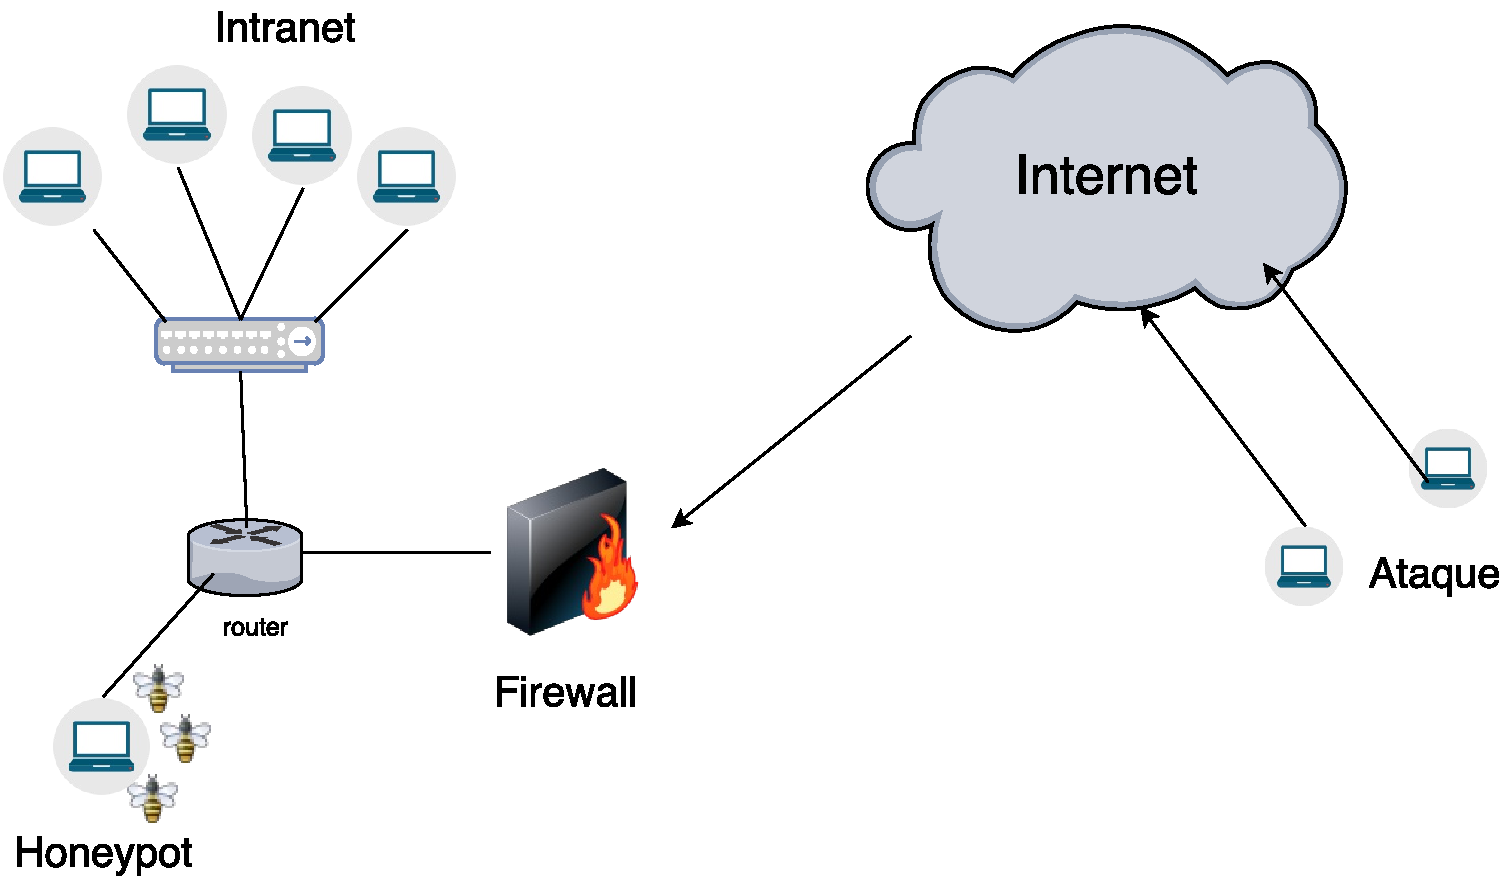
\includegraphics[width=0.9\textwidth]{pictures/honeypot.pdf}
        \caption{Honeypot}        
        \label{fig:honey}

    \end{figure}
    \FloatBarrier

\subsection{Honeynet}
\label{sec:honey1}

\COMMENT{Cuidado, uma honeynet é uma rede que abriga um conjunto de honeypots, geralmente distintos (por exemplo, usando sistemas operacionais diferentes). Essa discussão que você colocou aqui sobre a estrutura da rede pode aplicar-se quase da mesma forma a um honeypot isolado, pois ele precisa de elementos auxiliares para prover conectividade, monitorar e conter o tráfego.}

Uma \textit{Honeynet} é considera uma rede onde o \textit{Honeypot} está localizado, retratando os dispositivos que compõem esta estrutura. Uma \textit{Honeynet} pode estar composta por alguns elementos como: 

	\begin{itemize}
		\item A estrutura pode ser composta por diversos computadores;
		\item \textit{Firewall}, responsável pela realização de contenção e coleta de informações;
		\item IDS (Intrusion Detection System) tem o objetivo de observar a rede, buscando atividades em comum ou não autorizadas que podem danificar o sistema;
		\item roteadores, \textit{switches} e hubs para a composição da estrutura de rede \cite{honey:2007}%cite\ link
%http://www.cert.br/docs/whitepapers/honeypots-honeynets/
	\end{itemize}

O baixo custo e a interação do atacante com um ambiente real, contribuem com um estudo sobre as ferramentas utilizadas e vulnerabilidades exploradas.

\COMMENT{O parágrafo abaixo confunde conceitos. Uma honeynet virtual consiste em um conjunto de honeypots implementados em máquinas virtuais em um mesmo host físico (cf. \url{http://old.honeynet.org/papers/virtual/}); em uma honeynet real, cada honeypot é um host físico separado. Um honeypot/honeynet de pesquisa tem o propósito de estudar o comportamento dos atacantes; em contrapartida, um honeypot/honeynet de produção tem o objetivo de detectar ataques e responder a eles (cf. \url{http://www.it-docs.net/ddata/792.pdf}, p. 62). Acho que uma ideia aqui é pensar o que você \textbf{precisa} explicar para tornar o texto autocontido. Não vejo muito sentido em esmiuçar conceitos de honeypots e honeynets porque você não vai propor uma nova ferramenta, mas usar uma que já existe; o importante é que o leitor entenda o que é o DNSpot e suas principais características, e não que ele raciocine sobre as escolhas de projeto do DNSpot (isso compete ao TCC do Felipe).}

Existem duas classificações para os \textit{honeypots}, uma rede projetada especificamente para ser atacada e testada, visando a utilização de mecanismo de controle é conhecida como \textit{honeynet}, e uma rede com alta interatividade que busca obter informações dos usuários que estão realizando o ataque, também conhecida como \textit{honeynets virtuais} ou \textit{honeypot} de pesquisa \cite{honey:2007}.

\subsection{Aplicação}

Os \textit{honeypots} podem ser classificados em duas categorias, \textit{honeypot} de alta e baixa interatividade (como apresentado na \ref{sec:honey1}). O \textit{honeypot} de baixa interatividade busca identificar ataques internos e varreduras, também realiza identificação de máquinas comprometidas e códigos maliciosos. Já por outro lado o \textit{honeypot} de alta interatividade apresenta risco para a rede, podendo ser utilizado com o mesmo propósito do \textit{honeypot}  de baixa interatividade, seu principal objetivo é estudar o comportamento  detalhadamente dos atacantes, juntamente com técnicas e ferramentas utilizadas para explorar alguma vulnerabilidade \cite{honey:2007}.

 

\subsubsection{Aplicação na rede}    

%%%Utilização do honeynet

\section{DNSpot}
\label{sec:introDNSpot}

O DNSpot é um \textit{honeypot} projetado especificamente para monitorar e analisar o tráfego DNS \cite{Longo:2015:tcc}. Seu objetivo é permitir a observação das interações de usuários potencialmente maliciosos com servidores DNS recursivos. %%%felipe


\subsection{Definição}
\label{sec:defiDNSpot}

%%%%%%%FUNCIONAMENTO

\subsection{Arquitetura}
A arquitetura do DNSpot pode ser observada na figura \ref{fig:dnspot}. Ele possui um \textit{proxy} que escuta na porta 53/UDP, que é a porta padrão do serviço DNS\@. Ao receber uma consulta, o \textit{proxy} será responsável por armazenar a consulta em um banco de dados e logo em seguida repassá-la a um servidor DNS recursivo real. Esse servidor real, que aceita apenas consultas originadas na própria máquina, vai interagir com servidores autoritativos na Internet para a resolução desta consulta. Por último, o \textit{proxy} irá receber a resposta do servidor recursivo, armazená-la no banco de dados e encaminhá-la para o cliente que enviou a consulta \cite{Longo:2015:tcc}.


    \begin{figure}[ht]
        \centering
        \includegraphics[width=0.9\textwidth]{pictures/dnspot.png}
        \caption{Arquitetura DNSpot}        
        \label{fig:dnspot}

    \end{figure}
    \FloatBarrier


\COMMENT{O texto abaixo confunde dois mecanismos distintos. O SERVFAIL aleatório é para simular um servidor DNS inconfiável, tentando não levantar suspeitas caso o DNSpot seja desligado ou não consiga processar algumas consultas. Por sua vez, a limitação de consultas funciona como um mecanismo de contenção do tráfego gerado pelo DNSpot; ele permite que um usuário humano interaja com o honeypot, mas restringe a quantidade de tráfego gerada em caso de ataques de DoS por reflexão.}

O critérios de decisão escolhidos foram dois:

\begin{enumerate}

	\item Randomização: uma porcentagem é definida para as consultas, determinando se receberão uma resposta em tempo real ou não, e o \textit{proxy} faz uma decisão aleatória para determinar se será respondido a consulta ou será retornado um erro;

	\item Limitação: um limite diário é determinado para o número de consultas atendidas para cada endereço IP de origem; caso o limite seja atingido o \textit{proxy} passa a ignorar novas consultas do mesmo endereço,  até o dia seguinte (onde a atividade é retornada novamente) \cite{Longo:2015:tcc}.
	
\end{enumerate}

\section{Estatísticas}
\label{sec:introEsta}

\COMMENT{Acho que aqui você queria comentar os resultados do DNSpot, certo? Nesse caso, deveria ser uma \textit{subsection}, não uma \textit{section}.}

%%% Falar sobre a estatisticas e resultados 
%%%estatisticas DNSpot section
	\chapter{Trabalhos Relacionados}
\label{ch:relacionados}

%%%% COLOCAR ALGO AKI
Os trabalhos encontrados visam observar ataques DDoS em servidores raiz, ou a análise do comportamento de algumas características na rede. Existe diferenças nos períodos e tipos de análise realizadas.
 
Está seção busca apresentar algumas destas características e demonstrar algumas relações e diferenças com o trabalho apresentado. Dentre as diversas áreas de estudo sobre o DNS, como monitoramento, análise e detecção de anomalias



\section{Conceitualização}

\textbf{David Conrad} descreve primeiramente em seu trabalho \cite{Conrad:2012:tidssr}, conceitos para o entendimento do DNS e sua funcionalidade, ainda demonstrando uma conceitualização histórica. O trabalho demonstra a necessidade dos serviços do DNS para o funcionamento da \textit{Internet}, juntamente com todas as ameaças que este serviço possui.


\section{Análises}

\textbf{Roberto Perdisci} busca apresentar em seu trabalho \cite{DBLP:conf/acsac/PerdisciCDL09}


\section{Comparativo}

Para melhor entender as relações entre cada trabalho apresentando na seção \ref{ch:relacionados}, foi criado a tabela \ref{tab:all} onde é apresentando as principais características de cada trabalho.



%%%falar 4 artigos de análise dos ataques (pq a importância e oq cada análise focava fazer)

%%%terminar falando do tempo das análises para juntar com a proposta
    
%%%falar das análises que foram utilizados (relação das análise com relação ao tempo de coleta de dados) (subsection nova)

%%%falar qual foi o foco voltado dos trabalhos, a diferença para o meu trabalho (consigo falar do tempo) (período de análise dos dados principalmente, (subsection nova))



	\chapter{Proposta}
\label{ch:proposta}

O objetivo deste trabalho é desenvolver um estudo sobre a evolução temporal de dados coletados pelo DNSpot. Será levado em consideração as informações coletadas em um estudo anterior \cite{Longo:2015:tcc}.%citar o felipe.

O estudo observou interações de usuários potencialmente maliciosos com servidores DNS recursivos, observando a atitude tomada pelos usuários. A ferramenta foi implantada na rede da Universidade do Estado de Santa Catarina (UDESC), por um período de 49 dias.

Com as informações apresentadas pelo estudo \cite{Longo:2015:tcc}, será possível observar o surgimento de algumas características que não foram possíveis ser analisadas em um período de (49 dias). Possibilitando entender o comportamento de certos ataques não observados em outros estudos devido ao período que a análise foi proposta.

Levando em consideração os trabalhos apresentados na seção \ref{ch:relacionados}, é possível destacar os períodos de observação das redes, muitas das vezes por não serem desenvolvidos em períodos grandes de tempo, não é possível a realização de certas análise. Este trabalho busca apresentar uma análise em um período grande de tempo (6 meses), para a realização de uma análise evolucionária em relação aos dados observados.

Para efetuar a análise algumas modificações foram realizadas no DNSpot, focando em modificar algumas características do sistema, garantindo um melhor funcionamento em um período maior de tempo. Como relatado no trabalho  \cite{Longo:2015:tcc}, foram encontrados problemas devido ao crescimento do banco de dados, o que é um problema ao se realizar uma análise maior como a deste trabalho. 

A solução aborda foi a remoção de alguns campos que eram salvas no banco de dados, com isto o crescimento do banco foi controlado, mas ainda é possível observar que o banco vai apresentar um crescimento levando em consideração o período de análise. %citar o outro cara q eu n tenho o trabalho....

\subsection{Implantação}

%%%falar qual máquina está rodando
%%%Quando começou e até quando pretende ficar rodando a análise

Para a realização da coleta de dados, uma máquina foi disponibilizada pela UDESC. A máquina foi implantada na rede interna da universidade, onde está realizando a coleta de dados, que iniciaram no dia 17/09/2016. %OLHAR ESSA DATA...

A rede utiliza endereços reservados, por este motivo é necessário a utilização do NAT (Network Address Translation) para realizar o redirecionamento do tráfego para porta 53/UDP. O NAT é um método utilizado para remapear espaços de endereços IPs, realizando a modificação no cabeçalho dos pacotes no momento em que estes se encontram no dispositvo de roteamento \cite{Naugle:1998}. %cite o NAT

A configuração do \textit{hardware} e \textit{software} da máquina utilizada, segue:

\begin{itemize}
    \item Sistema Operacional: OpenBSD 5.7 i386;
    \item Processador: Intel Core2 Duo CPU E6550 @ 2.33GHz (``GenuineIntel" 686-class);
    \item Memória RAM: 1 GB;
    \item Servidor DNS recursivo: Unbound, versão 1.5.2;
    \item Python, versão 3.4.2;
    \item DNSLib, versão 0.9.4;
    \item SQLIte3, versão 3.8.6.
\end{itemize}


A máquina está localiza em um dos laboratórios da UDESC, onde realiza a coleta de dados 24/7, o serviço é verificado todos os dias para a garantia do seu funcionamento.

Durante o período que o sistema já esta executando as coletas, ocorreram algumas interrupções do serviço devido a queda de energia e interrupção do \textit{firewall} que da acesso a \textit{Internet} (consequencia da queda de energia).

\subsection{Tabelas no SQLite}

%http://stackoverflow.com/questions/784173/what-are-the-performance-characteristics-of-sqlite-with-very-large-database-file
%http://stackoverflow.com/questions/14451624/will-sqlite-performance-degrade-if-the-database-size-is-greater-than-2-gigabytes
%https://www.sqlite.org/limits.html


\subsection{Proposta de testes}
\label{sec:proposta_testes}

%%%falar as análises (discutir as análises dos artigos)

Levando em consideração os trabalhos apresentados na seção \ref{ch:relacionados}, e o trabalho realizado pelo \cite{Longo:2015:tcc}, foi determinar uma proposta de testes para este trabalho. A proposta leva em consideração algumas características observadas em trabalhos anteriores, e algumas propostas em comum, para realização de um comparativo entre os trabalhos.

Com os diferentes \textbf{períodos de monitoramento}, será possível realizar uma análise quanto a quantidade de informações capturadas em períodos diferentes. E realizar uma comparação entre a coleta realizada em um período inferior de tempo do \textit{Longo:2015:tcc}.


Com o total de \textbf{Transações} será possível realizar uma contagem do número de usuários com intenção maliciosa, já que é necessário a descoberta do endereço, como se trata de um servidor DNS não anunciado. Também será possível verificar o número de requisições que não foram respondidas e as transações ignoradas.

O \textbf{Volume de dados em bytes} ajudara para a descoberta dos tamanhos das consultas mais comuns juntamente com o tamanho das consultas e respostas solicitadas.

\textbf{Clientes IP}, para apresentar as localizações geográficas, juntamente com os endereços que realizaram o maior número de consultas. \textbf{Domínios} para o número de transações. Distribuição empírica de requisições por \textbf{RR} e número de transações.

\textbf{Ataques DoS} visando o tamanho de consulta e resposta, quantidade de ataques recebido.

\textbf{Anomalias} podem ser detectadas, levando em consideração os resultados já encontrados nos trabalhos anteriores \textit{Longo:2015:tcc}.

\textbf{Desaparecimento de domínios}, devido ao período estendido de análise será possível observar o surgimento e desaparecimento de muitos domínios, com os resultados é esperado conseguir um melhor entendimento deste comportamento devido ao período.



PRECISO REVISAR ISSO AKI	
	\makeatletter
\def\saveenum{\xdef\@savedenum{\the\c@enumi\relax}}
\def\resetenum{\global\c@enumi\@savedenum}
\makeatother

\chapter{Considerações Finais}
\label{ch:consideracoes}

Neste trabalho é apresentado o objetivo de realizar uma análise de um período grade (6 meses) de análise do tráfego, na Universidade do Estado de Santa Catarina. Após um estudo de trabalhos encontrados na área foi possível verificar que os períodos das análises registradas em períodos anteriores não são realizados em períodos grandes (maiores que um mes ou até mesmo dias), está trabalho foca em uma análise em um período maior de tempo (6 meses), com o objetivo de verificar o surgimento de alguns fatores/características que não foram observados devido ao período da análise destes outros trabalhos.

\section{O que foi feito}\label{sec:o_que_foi_feito}

No início deste período de estudo, que durou um total de três meses, foi realizado a formulação de um plano para o desenvolvimento deste trabalho, algumas das caracteríticas abordadas neste plano podem ser observadas como:

\begin{enumerate}[label=\textnormal{(\arabic*)}]
    \item Formulação do plano do TCC, especificação de algumas características para o início do trabalho;
    \item Revisão sobre DNS, \textit{honeypots} e DNSpot, para um melhor entendimento das principais características e funcionalidade da ferramenta que está sendo utilizada para a captura de informação;
    \item Revisão de trabalhos correlatos, identificação dos principais trabalhos relacionados com a pesquisa. Buscando analisar as análises utilizadas em outros trabalhos e o período que a pesquisa acabou ocorrendo. O principal fator analisado foi o período que as análises ocorreram;
    \item Adaptação no DNSpot para coletas de longo prazo, algumas modificações foram realizadas para que o DNSpot consiga lidar com o período de coleta, removendo algumas características que não torna-se essenciais para este estudo;
    \item Coleta de dados, o início da coleta de dados foi no dia 17/09/2016; %VERIFICAR ESSA DATA, LOG FILE TCC.....
    \item Definição das análises a serem realizadas, com um melhor entendimento e caracterização de alguns trabalhos na área, foi possível definir algumas características para a análise a ser realizada;
    \item Escrita da monografia da primeira parte (TCC-I).
\end{enumerate}


\section{Próximas etapas}\label{sec:proximas_etapas}


\begin{enumerate}[label=\textnormal{(\arabic*)}]
  \setcounter{enumi}{7}
    \item Análise dos resultados obtidos, com uma análise a longo prazo será possível observar algumas características e comportamentos não vistos em uma análise realizada em um período pequeno (um mes ou até mesmo dias);
    \item Escrita da monografia da segunda parte.
    \label{itm:1}
\end{enumerate}

\section{Cronograma}
\label{cro}

O cronograma proposto para a primeira etapa \ref{sec:o_que_foi_feito}, pode ser observador na tabela \ref{sec:consideracoes_cronograma}.

%%%% então acabei colocando ... mas acho q vou tirar HAHAH

\vspace{0.5cm}
{\tiny
\noindent \begin{tabular}{|c||c|c|c|c|c|c|c|c|c|c|c|c||c|c|c|c|c|c|c|c|c|c|c|c|}
  \hline
  \multirow{2}{*}{\textbf{\small{Etapas}}} & \multicolumn{12}{|c||}{\textbf{\small{2016}}} & \multicolumn{12}{|c|}{\textbf{\small{2017}}} \\
  \cline{2-25}
   & \textbf{J} & \textbf{F} & \textbf{M} & \textbf{A} & \textbf{M} & \textbf{J} & \textbf{J} & \textbf{A} & \textbf{S} & \textbf{O} & \textbf{N} & \textbf{D} & \textbf{J} & \textbf{F} & \textbf{M} & \textbf{A} & \textbf{M} & \textbf{J} & \textbf{J} & \textbf{A} & \textbf{S} & \textbf{O} & \textbf{N} & \textbf{D} \\
  \hline %\hline
  %\textbf{\small{1}} & & & & & & & x & x & & & & & & &  & & & & & & & & & \\
  \hline
  \textbf{\small{1}} & & & & & & & & x & x & & & & & & &  & & & & & & & & \\
  \hline
  \textbf{\small{2}} & & & & & & & &  & x & x & & & & & & & & & & & & & & \\
  \hline
  \textbf{\small{3}} & & & & & & & & & x & & & & & & & & & & & & & & & \\
  \hline
  \textbf{\small{4}} & & & & & & & & & & x & x & x & x & x & x & x & x
  & x & & & & & & \\
  \hline
  \textbf{\small{5}} & & & & & & & & & & x & x & & & & & & & & & & & & & \\
  \hline
  \textbf{\small{6}}  &  & & & & & & & & & & & & & x & x & x & x & x & & & & & & \\
  \hline
  \textbf{\small{7}} & & & & & & & & & & & & & & & & x & x & x & & & & & & \\
  \hline
%  \textbf{\small{9}} & & & & & & & & & & & & & & & & & x &  & & & & & & \\
%  \hline
%  \textbf{\small{10}} & & & & & & & & & & & & & & & & & x & x & x & & & & & \\
%  \hline  
%  \textbf{$\cdots$} & & & & & & & & & & & & & & & & & & & & & & & & \\
%  \hline
\end{tabular}
}

REFAZER ESSA TABELAAAAAA
\label{sec:consideracoes_cronograma}

	\bibliographystyle{abnt-alf}
\bibliography{refs}
	\appendix
\iffalse
\chapter{Apêndice: \textit{Datasets}}

%\section{\textit{Datasets}}
%\label{sec:revisao_datasets}

A seguir são listadas \textit{datasets} publicadas e que podem ser utilizadas para pesquisas. Para cada uma são detalhados o tipo (\textit{online} ou \textit{offline}), manuscrito ou impresso, o formato da informação, aonde encontrar os dados e a descrição.

\begin{itemize}
	\item detexify-data \cite{kirsch2010detexify}
	\subitem \textbf{Tipo}: \textit{Online}/manuscrito.
	\subitem \textbf{Formato}: Formato YAML $(x, y, time)$. Pontos espaçados com dados temporais.
	\subitem \textbf{Lincença}: ODbL (ODC \textit{Open Database License}).
	\subitem \textbf{Tamanho Aproximado}: $136042$ símbolos até janeiro de 2015.
	\subitem \textit{\textbf{Website}}: \url{https://github.com/kirel/detexify-data}
	\subitem \textbf{Descrição}: Os símbolos são dígitos, alfabeto latino minúsculo e maiúsculo, letras gregas e outros símbolos matemáticos.
	
	\item HWRT \cite{thoma2015line}
	\subitem \textbf{Tipo}: \textit{Online}/manuscrito.
	\subitem \textbf{Formato}: Formato YAML $(x, y, timestamp)$. Pontos espaçados com dados temporais.
	\subitem \textbf{Lincença}: ODbL (ODC \textit{Open Database License}).
	\subitem \textbf{Tamanho Aproximado}: $151158$ símbolos até janeiro de 2015.
	\subitem \textit{\textbf{Website}}: \url{http://www.martin-thoma.de/write-math/data}
	\subitem \textbf{Descrição}: Esta \textit{dataset} é composta por $90\%$ da \textit{detexify-data}. Os símbolos são dígitos, alfabeto latino minúsculo e maiúsculo, letras gregas e outros símbolos matemáticos.
	
	\item CROHME
	\subitem \textbf{Tipo}: \textit{Online}/manuscrito.
	\subitem \textbf{Formato}: Formato InkML. XML modificado que contém as expressões matemáticas em grupos de traços. Cada traço é composto por um conjunto de pontos. Cada ponto tem as coordenadas e o \textit{timestamp}.
	\subitem \textbf{Lincença}: \textit{Creative Commons license} para uso acadêmico. Proibido uso comercial.
	\subitem \textbf{Tamanho Aproximado}: ?
	\subitem \textit{\textbf{Website}}: \url{http://www.isical.ac.in/~crohme/CROHME_data.html}
	\subitem \textbf{Descrição}: \textit{Dataset} popular usada na competição CROHME reconhecimento de expressões matemáticas. Os dados são símbolos e expressões matemáticas inteiras.
	
	\item MfrDB \cite{stria2012mfrdb}
	\subitem \textbf{Tipo}: \textit{Online}/manuscrito.
	\subitem \textbf{Formato}: XML composto por InkML and MathML.
	\subitem \textbf{Lincença}: Gratuita para uso não comercial.
	\subitem \textbf{Tamanho Aproximado}: 2018 fórmulas matemáticas até janeiro de 2016.
	\subitem \textit{\textbf{Website}}: \url{http://mfr.felk.cvut.cz/Database_download.html}
	\subitem \textbf{Descrição}: 2018 fórmulas matemáticas escritas por 232 participantes por interface gráfica via \textit{mouse}, tela \textit{touch} ou \textit{stylus pen}.
	
%	\item MathBrush \cite{maclean2011grammar}
%	\subitem \textbf{Tipo}:
%	\subitem \textbf{Formato}: 
%	\subitem \textbf{Lincença}: 
%	\subitem \textbf{Tamanho Aproximado}: ?
%	\subitem \textit{\textbf{Website}}: \url{}
%	\subitem \textbf{Descrição}:
	
	\item HAMEX \cite{quiniou2011hamex}
	\subitem \textbf{Tipo}: \textit{Online}/manuscrito.
	\subitem \textbf{Formato}: InkML.
	\subitem \textbf{Lincença}: Não divulgada. Porém, Se entrar em contato eles disponibilizam.
	\subitem \textbf{Tamanho Aproximado}: 4350 expressões matemáticas.
	\subitem \textit{\textbf{Website}}: \url{http://ivc.univ-nantes.fr/en/databases/HAMEX}
	\subitem \textbf{Descrição}: Expressões matemáticas manuscritas e faladas (áudio).
	
	\item MNIST \cite{lecun1998gradient}
	\subitem \textbf{Tipo}: \textit{Offline}/manuscrito
	\subitem \textbf{Formato}: Formato IDX. Armazena vetores e matrizes com valores numéricos que representam a imagem de um dígito.
	\subitem \textbf{Lincença}: \textit{Creative Commons Attribution-Share Alike} 3.0.
	\subitem \textbf{Tamanho Aproximado}: 60 mil dígitos e mais 10 mil para o conjunto de testes.
	\subitem \textit{\textbf{Website}}: \url{http://yann.lecun.com/exdb/mnist}
	\subitem \textbf{Descrição}: \textit{Dataset} muito popular de dígitos $[0,9]$ manuscritos.
	
%	\item InftyCDB-1 \cite{suzuki2005ground}
%	\subitem \textbf{Tipo}: \textit{Offline}/printed.
%	\subitem \textbf{Formato}: ?
%	\subitem \textbf{Lincença}: ..
%	\subitem \textbf{Tamanho Aproximado}: ?
%	\subitem \textit{\textbf{Website}}: \url{http://www.inftyproject.org/en/database.html}
%	\subitem \textbf{Descrição}: Símbolos e fórmulas matemáticas impressas totalizando $21056$ expressões matemáticas.
	
	\item UW-III \cite{phillips1998methodologies}
	\subitem \textbf{Tipo}: \textit{Offline}/impresso.
	\subitem \textbf{Formato}: formato XFIG.
	\subitem \textbf{Lincença}: Proprietária.
	\subitem \textbf{Tamanho Aproximado}: 25 páginas impressas de fórmulas matemáticas.
	\subitem \textit{\textbf{Website}}: \url{http://isis-data.science.uva.nl/events/dlia/datasets/uwash3.html}
	\subitem \textbf{Descrição}: Essa base de dados é paga e custa USD 100.
	
	\item \cite{chajri2016handwritten}
	\subitem \textbf{Tipo}: \textit{Offline}/manuscrito.
	\subitem \textbf{Formato}: Imagens
	\subitem \textbf{Lincença}: ?
	\subitem \textbf{Tamanho Aproximado}: 10379 símbolos.
	\subitem \textit{\textbf{Website}}: \url{http://www.ncbi.nlm.nih.gov/pmc/articles/PMC4786757/}
	\subitem \textbf{Descrição}: $10379$ símbolos do alfabeto latino, árabe e símbolos matemáticos.
	
\end{itemize}


%\chapter{Apêndice: Ferramentas }

%aaa
%\section{Ferramentas relacionadas}
%\label{sec:revisao_ferramentas_relacionadas}

\fi
\end{document}
